%++++++++++++++++++++++++++++++++++++++++
% Don't modify this section unless you know what you're doing!
\documentclass[letterpaper,12pt]{article}
\usepackage{tabularx} % extra features for tabular environment
\usepackage{amsmath}  % improve math presentation
\usepackage{graphicx} % takes care of graphic including machinery
\usepackage[margin=1in,letterpaper]{geometry} % decreases margins
\usepackage{cite} % takes care of citations
\usepackage[latin9]{inputenc}
\usepackage{lmodern} % for writing code
\usepackage{tikz}
\usetikzlibrary{positioning,shapes.geometric}
\usepackage{minted}
\usepackage{amsfonts}


\usepackage[final]{hyperref} % adds hyper links inside the generated pdf file
\hypersetup{
	colorlinks=true,       % false: boxed links; true: colored links
	linkcolor=blue,        % color of internal links
	citecolor=blue,        % color of links to bibliography
	filecolor=magenta,     % color of file links
	urlcolor=blue         
}
\definecolor{ao(english)}{rgb}{0.0, 0.5, 0.0}
\usepackage{xcolor}
\renewcommand{\labelitemi}{$\bullet$}
\renewcommand{\labelitemii}{$\cdot$}
\renewcommand{\labelitemiii}{$\diamond$}
\renewcommand{\labelitemiv}{$\ast$}
%\usepackage[usenames,dvipsnames,svgnames,table]{xcolor}
%\let\oldtriangleleft\triangleleft
%\DeclareRobustCommand\bowtie{\mathrel\triangleright\joinrel\mathrel\oldtriangleleft}


%++++++++++++++++++++++++++++++++++++++++


\begin{document}

\title{Software Verification\\
Implementing a bounded model-checker}
\author{Ida Tucker}
\date{\today}
\maketitle

\begin{abstract}
The goal of this homework is to implement a bounded model-
checker based on a depth-first-search exploration of all the feasible paths
of the input program. Moreover, the SMT-solver Z3 will be used as an
execution engine to compute all the successive states along the explo-
ration. We will first present the global picture of it, then introduce a
few definition and semantics and, finally, list the steps you may follow
to implements the whole model-checking program.
\end{abstract}


\section{Implementation of Semantics.ml}
\paragraph{}
The \texttt{Semantics.ml} module translates the operators of the program into Z3 expressions in the integer theory module.
\subsection{Keeping track of formulas added to the Z3 expression}
\paragraph{}
In order to keep track of the formulas associated to each variable, a hashtable, global to the module, which is reset to zero for every new formula, is used. This hashtable \textit{\textcolor{blue}{ht}} binds the indexed program variables to the appropriate formula.
Seperate keys are added if the formula is asserting that a variable is non zero. These keys are of the form "\textit{x\$i non-zero}".
The hashtable has one additional key "\textit{guard}". If the program operation \textit{op} is a guard, the formula for the guard exists alongside the formulas added for each variable. Moreover we will only have one guard formula per operation.
\paragraph{}
Using a hashtable enables us to avoid the duplication of formulas associated to a given variable and to easily update them without having to check their existance. 
Thus the keys in the hashtable are:
\begin{itemize}
\item $\forall x \in X$,  \textcolor{purple}{x\$i}
\item $\forall x \in X$ such that we require $x \neq 0$, \textcolor{purple}{x\$inon-zero}
\item if \textit{op} is a guard, \textcolor{purple}{guard}
\end{itemize}

\subsection{Defining propositional formulas}
\paragraph{}
Now we have established how to keep track of the added formulas, let us see how they are built.
The commands are our program operations. In order to transform the program operation into a list of formulas we first need to determine what command is being applied.
Therefore, the \textcolor{blue}{formula} method pattern matches the input command \textit{\textcolor{blue}{cmd}} with the appropriate sort. According to the the matched sort, the appropriate function \textcolor{blue}{apply\_skip}, \textcolor{blue}{apply\_guard} or \textcolor{blue}{apply\_assign} is called. 

\begin{minted}{ocaml}
  match cmd with
  | Command.Skip ->
     List.iter (apply_skip ctx  i ) vars;
     Hashtbl.fold (fun _ v acc -> v :: acc) ht []
  | Command.Guard p ->
     apply_guard ctx p i vars;
     Hashtbl.fold (fun _ v acc -> v :: acc) ht []
  | Command.Assign (v, e) ->
     apply_assign ctx (v,e) i vars;
     Hashtbl.fold (fun _ v acc -> v :: acc) ht []
\end{minted}

If the program operation is \textit{skip}, seeing as the same formula will be applied to each variable we simply iterate through each variable in \textit{\textcolor{blue}{vars}} and apply skip. The \textcolor{blue}{apply\_skip} method (called on a single variable) ensures that the variable remains unchanged from index $i$ to index $i+1$ by adding a new formula to \textit{\textcolor{blue}{ht}} associated to $x^{(i)}$.

\paragraph{}
We will detail the \textcolor{blue}{apply\_guard} and \textcolor{blue}{apply\_assign} in \ref{guard} and \ref{assign}.
They both also update the hashtable and return \textit{unit}.
\paragraph{}
Whatever the program operation, after the appropriate function has been called, we iterate through the hashtable to build the returned list of formulas.

\subsection{Program operation is a guard}\label{guard}
If the command is a guard we have
\begin{align*}
op^{(i)} = g^{(i)} \wedge \bigwedge_{y \in X}y^{(i+1)} = y^{(i)}
\end{align*}
($ g^{(i)} = e_1^{(i)} \sim e_2^{(i)}$) where  $\sim$ is an operator in $ \{ = ,\leq, < , >, \geq \}$  

\paragraph{}
So we add a formula to our hashtable for the guard $g$, and for each variable we ensure that the variable remains unchanged from index $i$ to index $i+1$. 
Ensuring the variables remain unchanged is equivalent to calling \textcolor{blue}{apply\_skip} on all variables.
Thus the \textcolor{blue}{apply\_guard} function first adds a formula for the guard, before iterating through each variable in \textit{\textcolor{blue}{vars}}  and applying \textcolor{blue}{apply\_skip}.

The \textcolor{blue}{eval} function evaluates the expressions $e_1^{(i)}$ and $e_2^{(i)}$ recursively, in order to build formulas in the Z3 context for the expressions. The eval function takes care of adding a \textcolor{purple}{non-zero} key to \textit{\textcolor{blue}{ht}} if the expression includes a division by a program variable (or by an expression including program variables).

\subsection{Program operation is an assignment}\label{assign}

If the command is an assignment we have:
\begin{align*}
op^{(i)} = (x^{(i+1)} = e^{(i)}) \wedge \bigwedge_{y \in X\backslash \{x\} }(y^{(i+1)} = y^{(i)})
\end{align*}

All variables should remain unchanged from index $i$ to index $i+1$ \textit{except} the variable that is being assigned to. Thus \textcolor{blue}{apply\_assign} iterates through each variable in \textit{\textcolor{blue}{vars}} and applies \textcolor{blue}{apply\_skip} before adding a formula for the assignment asociated with $x^{(i)}$, which will replace the previous binding of $x^{(i)}$.

i.e. the binding \textcolor{purple}{x\$i}, $x^{(i)}$ = $x^{(i+1)}$ becomes \textcolor{purple}{x\$i}, $x^{(i+1)} = e^{(i)}$.

In order to build the assignment formula we match the expression assigned to $x^{(i)}$ with either a constant, another variable or an expression. Again if $e$ is an expression we use the \textcolor{blue}{eval} function to evaluate the expression.

  
\section{Implementation of BoundedModelChecking.ml}
\subsection{Marking locations as visited}
In order to keep a reccord of which locations have already been visited by the depth first search performed by this module, the hashtable \texttt{visited\_ht}, global to the module, binds a location to the value 1 when it is visited. On entering the \texttt{\textcolor{blue}{depth\_first\_search}} function, if the current location has been visited, no action is taken and the function returns unit. If the location has not yet been visited we propagate our depth first search.


\subsection{Kepping track of path and depth of search}

\begin{itemize}
\item The gobal variable \texttt{depth} is incremented every time we apply \texttt{\textcolor{blue}{depth\_first\_search}} to a child node.
\item The gobal variable \texttt{path} is a list of pairs \texttt{(command, location)} that keeps track of the edges of the CFA taken to get to the current location.
\item The gobal variable \texttt{bad\_path} is a list of pairs \texttt{(command, location)} that lead to the final location, if such a path of depth lower than \texttt{bound} exists. If no such path exists (or has been discoverred yet) \texttt{bad\_path} is the empty list.
\item \texttt{bound\_reached} is a boolean, initally set to \texttt{false}, to which we assign the value \texttt{true} if there exists a path along which the bound is reached before encountering the final location or an unreachable location.
\end{itemize}


\subsection{Building the path and the path formula}
\paragraph{}
Every time a new branch of the CFA is explored, the \texttt{\textcolor{blue}{depth\_first\_search}} function checks if the location has been visited, if so it returns, if not it marks the location as visited. 

Next it checks if \texttt{bad\_path} is empty, if not it returns. 

If \texttt{bad\_path} is empty, it checks if the \texttt{bound} has been reached, if so it returns.

Otherwise we are in the valid situation where the program should continue the depth first search. In this situation the following logic is applied:

\begin{itemize}
\item Create a new scope for the solver by saving the current stack size: pushing the solver will enable us to backtrack later on if we reach the \texttt{bound} or an unfeasible path.
\item Call \texttt{\textcolor{blue}{Semantics.}formula} on the program operation for the current depth in order to convert the command into a propositional logic formula.
\item Add the formula to the solver.
\item Add the pair \texttt{(command, location)} to the \texttt{path} list.
\item Check the satisfiability of the solver. At this point, three situations may arrise:
\begin{enumerate}
\item{The solver is not satisfiable, in which case we backtrack:
\begin{itemize}
\item restore the previous context by popping the solver
\item decrease the depth by one
\item remove the last pair \texttt{(command, location)} that was added to \texttt{path}
\item return \texttt{unit}.
\end{itemize}
}
\item The solver is satisfiable and we have reached the final location. In this case we assign \texttt{path} to \texttt{bad\_path} and return \texttt{unit}.
\item The solver is satisfiable, thus the location is reachable, and the location is not the final location. In this situation we iterate through all locations accessible from the current location and apply \texttt{\textcolor{blue}{depth\_first\_search}}.
\end{enumerate}
\end{itemize}

\subsection{Searching for a path to the final state}
\paragraph{}
The \texttt{\textcolor{blue}{search}} function brings all the above functionality together.
It first initialises the global variables before calling \texttt{\textcolor{blue}{depth\_first\_search}} on the initial location with the command skip.

If after calling \texttt{\textcolor{blue}{depth\_first\_search}} the \texttt{bad\_path} list is not empty, then the depth first search found a feasible path to the final location and we return \texttt{Path bad\_path}.

If no path to the final state was found, and if the bound was reached, we do not know if the program is safe, we only know that there is no path to the final state in less than \texttt{bound} steps. In this case the \texttt{bound\_reached} variable is true, and we return \texttt{Empty \textcolor{teal}{false}}.

Otherwise, all feasible paths of have been explored and none lead to the final state. The program is safe and we return \texttt{Empty \textcolor{teal}{true}}.


\section{Tests}
Added test to \texttt{semantics.assign} for the division of an expression by a constant. We add a formula that asserts the integer constant is non zero.
\begin{minted}{ocaml}
[z := (x / 2)]^1: expects `{(= z$2 (div x$1 2)), (= x$1 x$2),
				(= y$1 y$2), (not (= 2 0))}'
\end{minted}
Added test to \texttt{semantics.assign} for the division of an expression by an expression that is neither a constant nor a variable.
\begin{minted}{ocaml}
[z := (x / (y + 3))]^1: expects `{(= z$2 (div x$1 (+ y$1 3))), (= x$1 x$2),
				(= y$1 y$2), (not (= (+ y$1 3) 0))}'
\end{minted}

\subsection{New Automatons}
For testing purposes, additional automatons have been created in the \texttt{examples} folder in order to test edge cases, the case where no feasible path is found in less than 10 iterations, potential infinite loops.

\subsubsection{Initial state is bad state}
\paragraph{Test}
This tests the edge case where the initial and final location are the same node.
\paragraph{Expected result}
We expect a feasible path that is simply the initial location (no commands).
\paragraph{Obtained result}
\textbf{\textcolor{teal}{PASS}}


\subsubsection{Initial state skips to bad state}
\paragraph{Test}
This tests the edge case where the initial location skips to the final location.
\paragraph{Expected result}
We expect a feasible path that is simply a skip from the initial location to the final location.
\paragraph{Obtained result}
\textbf{\textcolor{teal}{PASS}}

\subsubsection{Looping until reaching the final location}
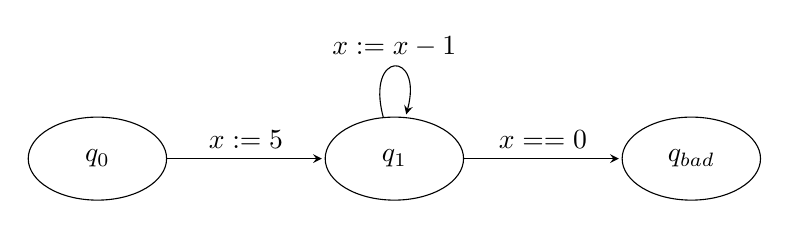
\begin{tikzpicture}[%
    ->,shorten >=1pt,>=stealth,node distance=7cm,noname/.style={%
      ellipse,minimum width=5em, minimum height=3em,draw}
  ]
    \node[noname] (ini)                                                {$q_{0}$};
    \node[noname] (1) [node distance=2cm, right=of ini]    {$q_{1}$};
    \node[noname] (bad) [node distance=2cm, right=of 1]   {$q_{bad}$};
    \path (ini) edge [above]                  node {$x:=5$} (1)
    	  (1)   edge [loop above]             node {$x:=x-1$} (1)
          (1)   edge [above]                  node {$x==0$} (bad)
          ;
  \end{tikzpicture}
\paragraph{Test:}
Ensuring that the program will loop on a single state in order to reach the final node.
\paragraph{Expected result:}
We exepct bounded model checker to find a path to the final state.

\paragraph{Obtained result:}

\begin{minted}{ocaml}
Feasible path:
   q_0
      >> x := 5 >>
   q_1
      >> x := (x - 1) >>
   q_1
      >> x := (x - 1) >>
   q_1
      >> x := (x - 1) >>
   q_1
      >> x := (x - 1) >>
   q_1
      >> x := (x - 1) >>
   q_1
      >> x == 0 >>
   q_2

\end{minted}

\textbf{\textcolor{teal}{PASS}}

\subsubsection{Limit under and limit over \texttt{bound}}
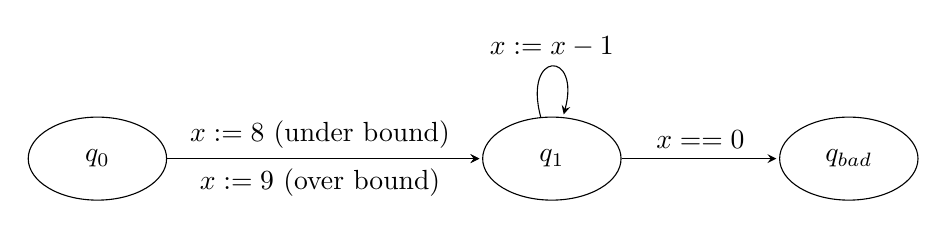
\begin{tikzpicture}[%
    ->,shorten >=1pt,>=stealth,node distance=7cm,noname/.style={%
      ellipse,minimum width=5em, minimum height=3em,draw}
  ]
    \node[noname] (ini)                                                {$q_{0}$};
    \node[noname] (1) [node distance=4cm, right=of ini]    {$q_{1}$};
    \node[noname] (bad) [node distance=2cm, right=of 1]   {$q_{bad}$};
    \path (ini) edge [above]                  node {$x:=8 \mbox{ (under bound) }$} (1)
    	  (ini) edge [below]                  node {$x:=9 \mbox{ (over bound) }$} (1)
    	  (1)   edge [loop above]             node {$x:=x-1$} (1)
          (1)   edge [above]                  node {$x==0$} (bad)
          ;
  \end{tikzpicture}
\paragraph{Test:}
These tests check that if the CFA requires exactly 10 steps to the bad state then the \texttt{bad\_path} is found, if it requires one more step then no feasible path of length $\leq 10$ is found.
\paragraph{Expected result:}
Limit under bound should find a path to the final state.
Limit over bound should find no feasible path of length $\leq 10$.
\paragraph{Obtained result:}
\textbf{\textcolor{teal}{PASS}}

  
\subsubsection{Always negative}
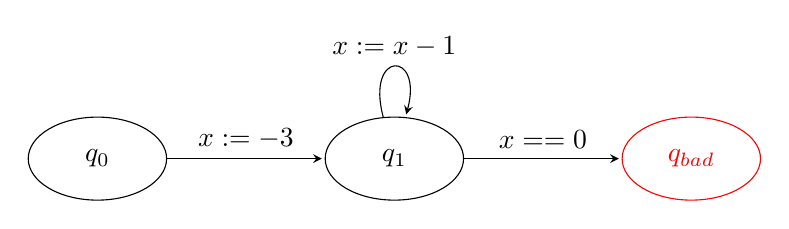
\begin{tikzpicture}[%
    ->,shorten >=1pt,>=stealth,node distance=7cm,noname/.style={%
      ellipse,minimum width=5em, minimum height=3em,draw}
  ]
    \node[noname] (ini)                                        {$q_{0}$};
    \node[noname] (1) [node distance=2cm, right=of ini]        {$q_{1}$};
    \node[noname, red] (bad) [node distance=2cm, right=of 1]   {$q_{bad}$};
    \path (ini) edge [above]                  node {$x:=-3$}  (1)
    	  (1)   edge [loop above]             node {$x:=x-1$} (1)
          (1)   edge [above]                  node {$x==0$}   (bad)
          ;
  \end{tikzpicture}
\paragraph{Test}
Ensure the above automaton cannot find a bad path, since we have a safe inductive invariant:
\begin{itemize}
\item $\varphi _{q_0}$ = true
\item $\varphi _{q_1}$ = $ x < 0$
\item $\varphi _{q_{bad}}$ = false
\end{itemize}
\paragraph{Expected result:}
No path to the final state should be found.
\paragraph{Obtained result:}
The bounded model checker does not garantee the safety of the the pogram but whatever the \texttt{bound} set, it finds no feasible path to the error state of length $\leq$ \texttt{bound}.
\textbf{\textcolor{teal}{PASS}}

\subsubsection{Unsafe program}
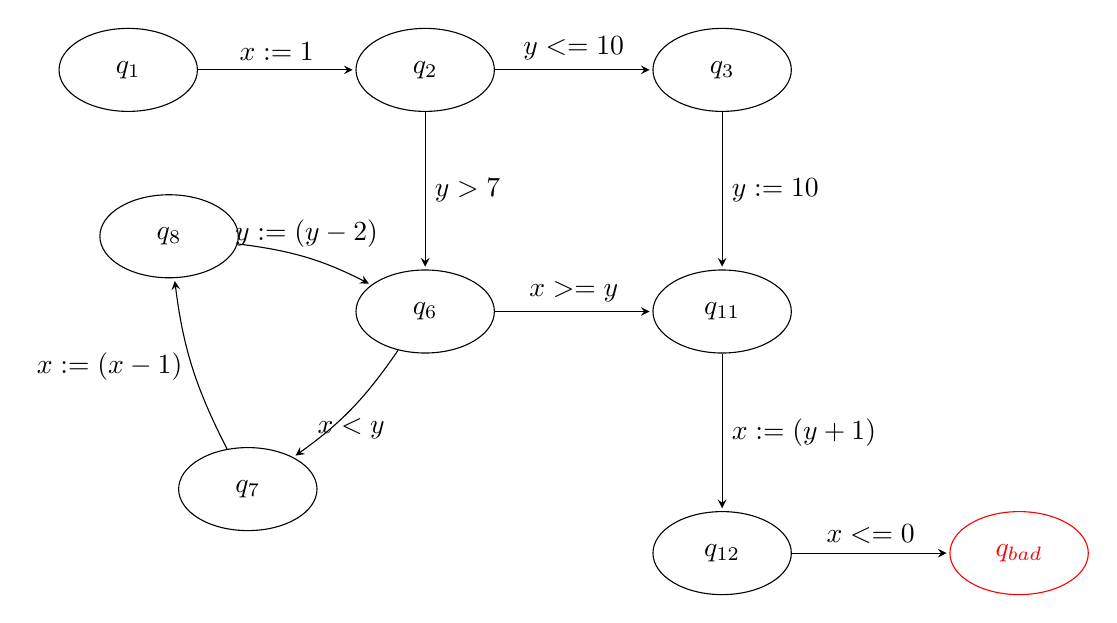
\begin{tikzpicture}[%
    ->,
    shorten >=1pt,
    >=stealth,
    node distance=7cm,
    noname/.style={%
      ellipse,
      minimum width=5em,
      minimum height=3em,
      draw
    }
  ]
    \node[noname] (1)                                   {$q_{1}$};
    \node[noname] (2) [node distance=2cm,right=of 1]    {$q_{2}$};
    \node[noname] (3) [node distance=2cm,right=of 2]    {$q_{3}$};
    \node[noname] (6) [node distance=2cm,below=of 2]    {$q_{6}$};
    \node[noname] (7) [node distance=1.5cm and 1cm,below left=of 6]    {$q_{7}$};
    \node[noname] (8) [node distance=0.2cm and 2,above left=of 6]    {$q_{8}$};
    \node[noname] (11) [node distance=2cm,below =of 3]   {$q_{11}$};
    \node[noname] (12) [node distance=2cm,below=of 11]   {$q_{12}$};
    \node[noname, red] (bad) [node distance=2cm,right=of 12]   {$q_{bad}$};

    \path (1) edge  [above]                  node {$x := 1$}   (2)
          (2) edge  [above]                  node {$y <= 10$}  (3)
          (2) edge  [right]                  node {$y >7$}    (6)
          (3) edge  [right]                  node {$y := 10$}  (11)
          (6) edge  [bend left=10pt, below]  node {$x < y$}    (7)
          (6) edge  [above]                  node {$x >= y$}   (11) 
          (7) edge  [bend left=10pt, left]   node {$x := (x-1)$} (8)
          (8) edge  [bend left=10pt, above]  node {$y := (y-2)$} (6)
          (11) edge [right]                  node {$x := (y+1)$} (12)
          (12) edge [above]                  node {$x <= 0$}     (bad)
          ;
  \end{tikzpicture}
\paragraph{Test}
This tests that for a slightly more complex unsafe program, the bounded model checker finds a path to the final state.

\paragraph{Expected result}
We expect a feasible path that is simply a skip from the initial location to the final location. However only for a big enough bound.
\paragraph{Obtained result}
For a bound of 26 a feasible path is found.

\textbf{\textcolor{teal}{PASS}}

\subsubsection{Recognizing fixed points}
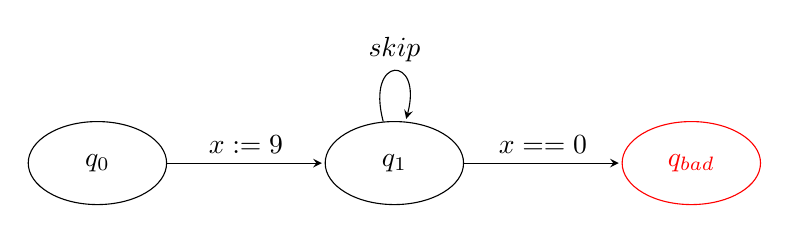
\begin{tikzpicture}[%
    ->,shorten >=1pt,>=stealth,node distance=7cm,noname/.style={%
      ellipse,minimum width=5em, minimum height=3em,draw}
  ]
    \node[noname] (ini)                                        {$q_{0}$};
    \node[noname] (1) [node distance=2cm, right=of ini]        {$q_{1}$};
    \node[noname, red] (bad) [node distance=2cm, right=of 1]   {$q_{bad}$};
    \path (ini) edge [above]                  node {$x:=9$}  (1)
    	  (1)   edge [loop above]             node {$skip$} (1)
          (1)   edge [above]                  node {$x==0$}   (bad)
          ;
  \end{tikzpicture}
\paragraph{Test}
This tests that the bounded model checker does not get stuck in an infinite loop if the state is the same as a peviously encountered one. Therefore if a location has been visited and the solver obtained when reaching this location is equivalent to a solver previously obtained at this location, do not propagate the depth first search.

\paragraph{Expected result}
We expect the program to be proved as safe, as iterating the loop does not change the state of the program.
\paragraph{Obtained result}
No path of length $\leq$ \texttt{bound} is found.
 
\textbf{\textcolor{red}{FAIL}}

\subsection{Existing Automaton examples}
\subsubsection{Division by zero}
The division by zero automaton should not lead to a bad state, indeed 
\begin{itemize}
\item $q_{ini} \rightarrow q_1 $: enforces $x:=-1$, so we cannot have $y:=\frac{3}{x+1}$ we would have a division by zero, this produces an UNSAT formula.
\item $q_{ini} \rightarrow q_2 $: enforces $x:=\frac{x}{y+2}$, so we cannot have $y==-2$.
\item $q_{ini} \rightarrow q_3 $: enforces $\frac{x}{y} > 3$, so we must have $y\neq 0$.
\item $q_{ini} \rightarrow q_{bad} $: dividing by zero produces an UNSAT formula.
\end{itemize}  

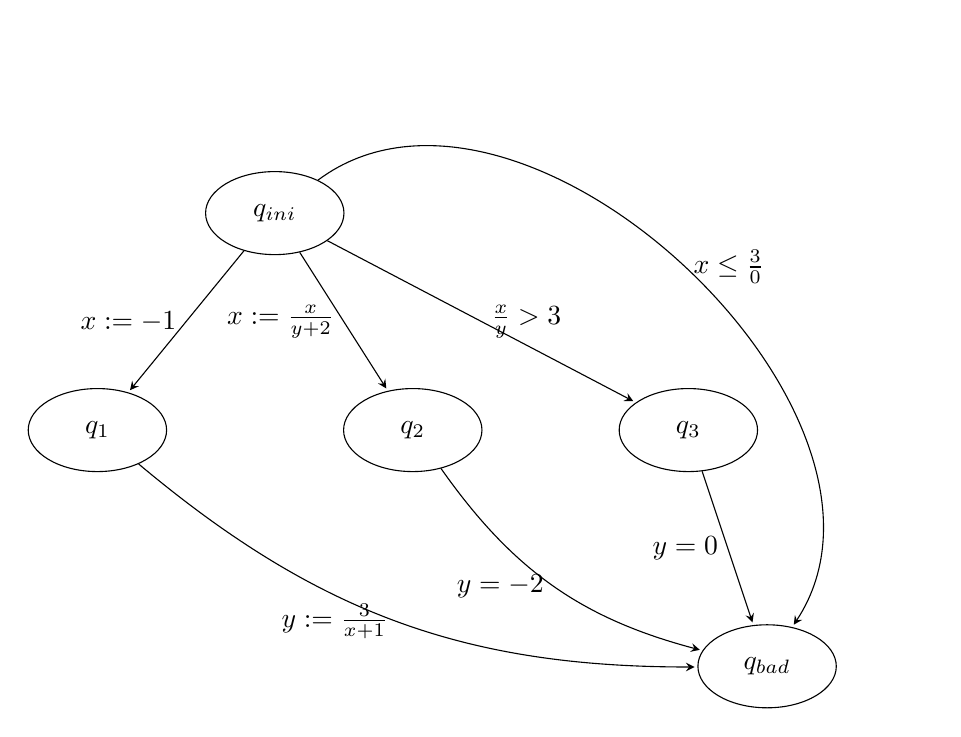
\begin{tikzpicture}[%
    ->,
    shorten >=1pt,
    >=stealth,
    node distance=7cm,
    noname/.style={%
      ellipse,
      minimum width=5em,
      minimum height=3em,
      draw
    }
  ]
    \node[noname] (ini)                                                {$q_{ini}$};
    \node[noname] (1) [node distance=2cm and 1cm,below left=of ini]    {$q_{1}$};
    \node[noname] (2) [node distance=2cm and 0.5cm,below right=of ini] {$q_{2}$};
    \node[noname] (3) [node distance=2cm and 4cm,below right=of ini]   {$q_{3}$};
    \node[noname] (bad) [node distance=5cm and 5cm,below right=of ini]   {$q_{bad}$};

    \path (ini) edge [left]                  node {$x:=-1$} (1)
          (ini) edge [left]                  node {$x:=\frac{x}{y+2}$} (2)
          (ini) edge [right]                  node {$\frac{x}{y} > 3$} (3)
          (ini) edge [bend left=80pt, right] node {$x \leq \frac{3}{0}$} (bad)
          (1)   edge [bend right=20pt, left] node {$y:=\frac{3}{x+1}$} (bad)
          (2)   edge [bend right=20pt, left] node {$y = -2$} (bad)
          (3)   edge [left] node {$y=0$} (bad)
          ;
  \end{tikzpicture}

\subsubsection{Constant Propagation}

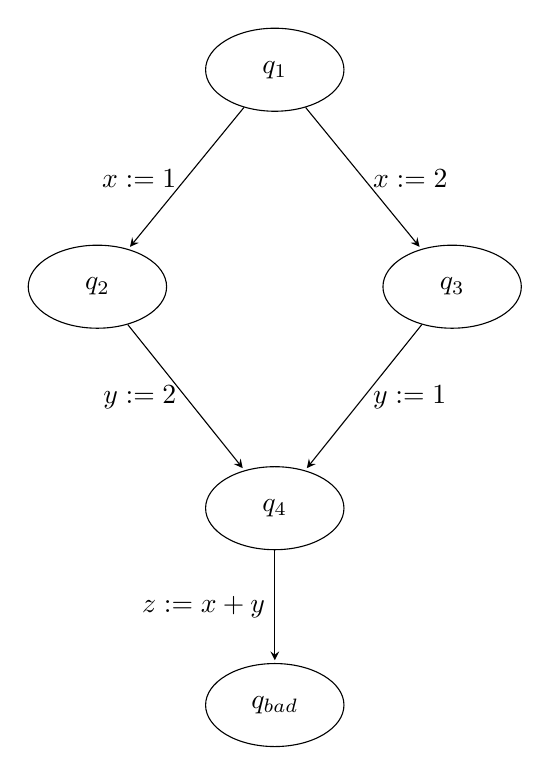
\begin{tikzpicture}[%
    ->,
    shorten >=1pt,
    >=stealth,
    node distance=7cm,
    noname/.style={%
      ellipse,
      minimum width=5em,
      minimum height=3em,
      draw
    }
  ]
    \node[noname] (1)                                                {$q_{1}$};
    \node[noname] (2) [node distance=2cm and 1cm,below left=of 1]    {$q_{2}$};
    \node[noname] (3) [node distance=2cm and 1cm,below right=of 1] {$q_{3}$};
    \node[noname] (4) [node distance=4.5cm,below =of 1]   {$q_{4}$};
    \node[noname] (bad) [node distance=7cm,below =of 1]   {$q_{bad}$};

    \path (1) edge [left]                   node {$x:=1$}   (2)
          (1) edge [right]                  node {$x:=2$}   (3)
          (2) edge [left]                   node {$y:=2$}   (4)
          (3) edge [right] 					node {$y:=1$}   (4)
          (4) edge [left]  					node {$z:=x+y$} (bad)
          ;
  \end{tikzpicture}

Clearly the constant propagation automaton is unsafe: for any initial value of x and y and for z=3, the final state $q_{bad}$ is reached. The program finds the following feasible path to $q_{bad}$:

\begin{minted}{c}
Feasible path:
   q_1
     >> x := 1 >>
   q_2
      >> y := 2 >>
   q_4
      >> z := (x + y) >>
   q_5

\end{minted}


\subsubsection{Inductive Invariants Exercise 1}
\begin{tikzpicture}[%
    ->,
    shorten >=1pt,
    >=stealth,
    node distance=7cm,
    noname/.style={%
      ellipse,
      minimum width=5em,
      minimum height=3em,
      draw
    }
  ]
    \node[noname] (0)                                      {$q_{0}$};
    \node[noname] (1)   [node distance=3cm, right=of 0]    {$q_{1}$};
    \node[noname] (bad) [node distance=8cm, right=of 0]    {$q_{bad}$};

    \path (0) edge [above]                    node {$x:=0$}       (1)
          (1) edge [loop above=80pt,above]    node {$x:=(x*y)$}   (1)
          (1) edge [loop below=100pt, below]  node {$x:=(x+3)$}   (1)
          (1) edge [above]  				  node {$x==10$}     (bad)
          ;
  \end{tikzpicture}
  
In this exercise we have a safe inductive invariant:
\begin{itemize}
\item $\varphi _{q_0}$ = true
\item $\varphi _{q_1}$ = $\exists k \in \mathbb{Z} : x = 3*k$
\item $\varphi _{q_{bad}}$ = false
\end{itemize}

The bounded model checker finds that there is no feasible path of length $<= 10$.

\textbf{\textcolor{teal}{PASS}}

\subsubsection{Inductive Invariants Exercise 2}

\begin{tikzpicture}[%
    ->,
    shorten >=1pt,
    >=stealth,
    node distance=7cm,
    noname/.style={%
      ellipse,
      minimum width=5em,
      minimum height=3em,
      draw
    }
  ]
    \node[noname] (0)                                                {$q_{0}$};
    \node[noname] (1) [node distance=2cm,right=of 0]    {$q_{1}$};
    \node[noname] (2) [node distance=2cm,right=of 1] {$q_{2}$};
    \node[noname] (3) [node distance=2cm,right=of 2]   {$q_{3}$};
    \node[noname] (4) [node distance=2cm,below=of 2]   {$q_{4}$};
    \node[noname, red] (bad) [node distance=2cm,left=of 4]   {$q_{bad}$};

    \path (ini) edge [above]                  node {$y > 0$} (1)
          (1) edge [above]                    node {$x:=0$} (2)
          (2) edge [bend right=20pt,below]     node {$x:= (x+y)$} (3)
          (2) edge [right]   node {$y==0$} (4)
          (3) edge [bend right=20pt, above]   node {$y:=(y-1)$} (2)
          (4) edge [above]   node {$x==0$} (bad)
          ;
  \end{tikzpicture}

In this exercise we have a safe inductive invariant:
\begin{itemize}
\item $\varphi _{q_0}$ = true
\item $\varphi _{q_1}$ = $y > 0$
\item $\varphi _{q_2}$ = $(y>0 \Rightarrow x \geq 0) \wedge (y=0 \Rightarrow x>0)$
\item $\varphi _{q_3}$ = $(y\geq 0 \Rightarrow x > 0)$
\item $\varphi _{q_4}$ = $(y=0 \wedge x > 0)$
\item $\varphi _{q_{bad}}$ = false
\end{itemize}

The bounded model checker finds that there is no feasible path of length $<= 10$.

\textbf{\textcolor{teal}{PASS}}

\subsubsection{Running Example}
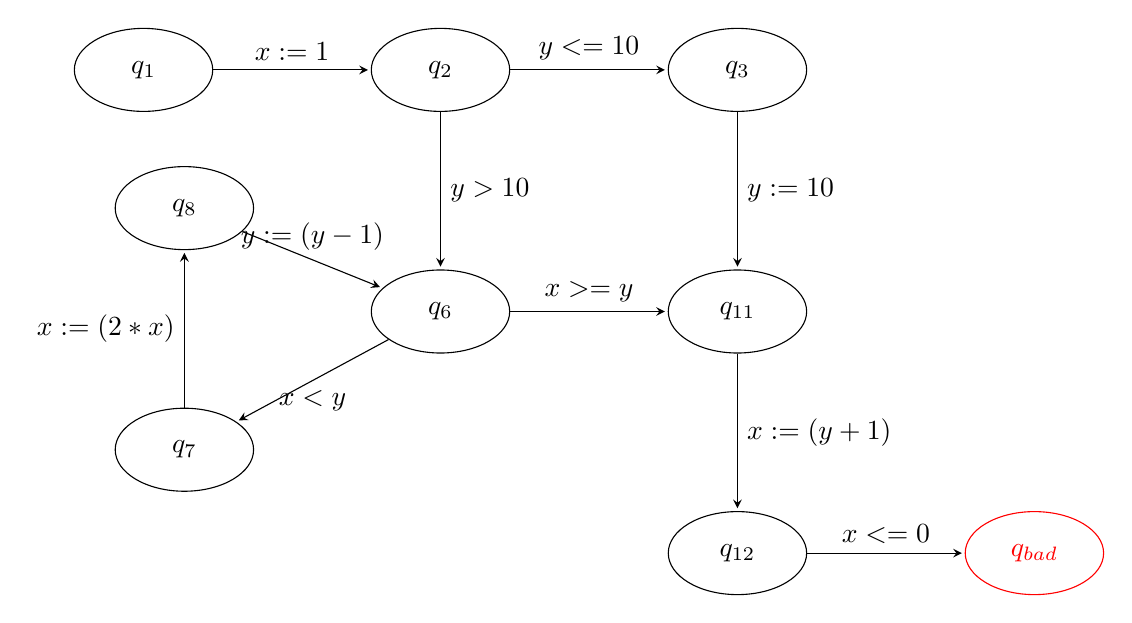
\begin{tikzpicture}[%
    ->,
    shorten >=1pt,
    >=stealth,
    node distance=7cm,
    noname/.style={%
      ellipse,
      minimum width=5em,
      minimum height=3em,
      draw
    }
  ]
    \node[noname] (1)                                   {$q_{1}$};
    \node[noname] (2) [node distance=2cm,right=of 1]    {$q_{2}$};
    \node[noname] (3) [node distance=2cm,right=of 2]    {$q_{3}$};
    \node[noname] (6) [node distance=2cm,below=of 2]    {$q_{6}$};
    \node[noname] (7) [node distance=1cm and 2cm,below left=of 6]    {$q_{7}$};
    \node[noname] (8) [node distance=2cm,above=of 7]    {$q_{8}$};
    \node[noname] (11) [node distance=2cm,below =of 3]   {$q_{11}$};
    \node[noname] (12) [node distance=2cm,below=of 11]   {$q_{12}$};
    \node[noname, red] (bad) [node distance=2cm,right=of 12]   {$q_{bad}$};

    \path (1) edge [above]                  node {$x:=1$} (2)
          (2) edge [above]                  node {$y<=10$} (3)
          (2) edge [right]                  node {$y>10$} (6)
          (3) edge [right]   node {$y:=10$} (11)
          (6) edge [below]   node {$x<y$} (7)
          (6) edge [above]   node {$x>=y$} (11) 
          (7) edge [left]   node {$x:=(2*x)$} (8)
          (8) edge [above]   node {$y:=(y-1)$} (6)
          (11) edge [right]   node {$x:= (y+1)$} (12)
          (12) edge [above]   node {$x<=0$} (bad)
          ;
  \end{tikzpicture}
  
With extended sign analysis we proved that this program is safe. The bounded model checker finds that there is no feasible path of length $<= 10$.

\textbf{\textcolor{teal}{PASS}}

\subsubsection{Infinite Descent}

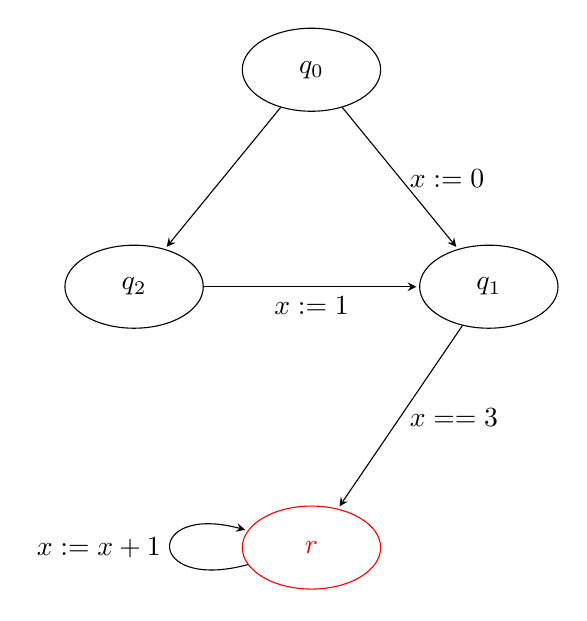
\begin{tikzpicture}[%
    ->,
    shorten >=1pt,
    >=stealth,
    node distance=7cm,
    noname/.style={%
      ellipse,
      minimum width=5em,
      minimum height=3em,
      draw
    }
  ]
    \node[noname] (0)                                                {$q_{0}$};
    \node[noname] (1) [node distance=2cm and 1cm,below right=of 0]   {$q_{1}$};
    \node[noname] (2) [node distance=2cm and 1cm,below left=of 0]    {$q_{2}$};
    \node[noname, red] (bad) [node distance=5cm,below=of 0]          {$r$};

    \path (0) edge []                    node {}       (2)
          (0) edge [right]                    node {$x:=0$} (1)
          (1) edge [right]    node {$x == 3$} (bad)
          (2) edge [below]                    node {$x:=1$} (1)
          (bad) edge [loop left]                    node {$x:=x+1$} (bad)
          ;
  \end{tikzpicture}
  
Clearly this automaton has no feasible path, we have a safe inductive invariant:
\begin{itemize}
\item $\varphi _{q_0}$ = true
\item $\varphi _{q_1}$ = $(x=0) \vee (x=3)$
\item $\varphi _{q_2}$ = true
\item $\varphi _{q_{bad}}$ = false
\end{itemize}   
The bounded model checker also finds that there is no feasible path.

\textbf{\textcolor{teal}{PASS}}
\subsubsection{Pre Only}

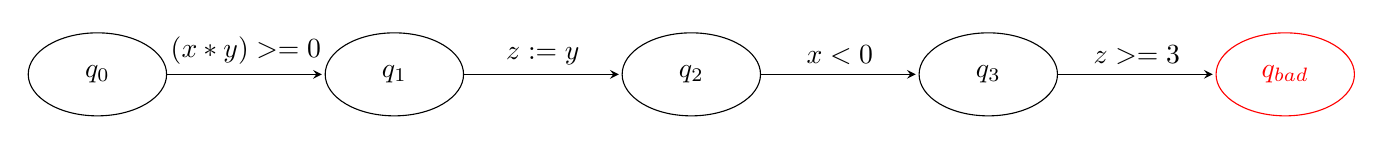
\begin{tikzpicture}[%
    ->,
    shorten >=1pt,
    >=stealth,
    node distance=7cm,
    noname/.style={%
      ellipse,
      minimum width=5em,
      minimum height=3em,
      draw
    }
  ]
    \node[noname] (0)                                                {$q_{0}$};
    \node[noname] (1) [node distance=2cm, right=of 0]   {$q_{1}$};
    \node[noname] (2) [node distance=2cm, right=of 1]    {$q_{2}$};
    \node[noname] (3) [node distance=2cm, right=of 2]    {$q_{3}$};
    \node[noname, red] (bad) [node distance=2cm,right=of 3]          {$q_{bad}$};

    \path (0) edge [above]                    node {$(x*y) >= 0$}       (1)
          (1) edge [above]                    node {$z:=y$} (2)
          (2) edge [above]                     node {$x<0$} (3)
          (3) edge [above]                    node {$z>=3$} (bad)
          ;
  \end{tikzpicture}

Again we have a safe inductive invariant:
\begin{itemize}
\item $\varphi _{q_0}$ = true
\item $\varphi _{q_1}$ = $((x\geq 0) \wedge (y\geq 0)) \vee ((x\leq 0 )\wedge( y\leq 0))$
\item 
$\varphi _{q_2}$ = $((x\geq 0) \wedge (y\geq 0)) \vee ((x\leq 0 )\wedge( y\leq 0)) \bigwedge (z=y)$ \\
$\Leftrightarrow \varphi _{q_2}$ =$((x\geq 0) \wedge (z\geq 0)) \vee ((x\leq 0 )\wedge( z\leq 0)) \bigwedge (z=y)$
\item $\varphi _{q_3}$ = $((x < 0 )\wedge( z\leq 0)) \bigwedge (z=y)$
\item $\varphi _{q_{bad}}$ = false
\end{itemize}   

The bounded model checker also finds that there is no feasible path.

\textbf{\textcolor{teal}{PASS}}

\subsubsection{Sign Non Zero Crucial}
\begin{tikzpicture}[%
    ->,
    shorten >=1pt,
    >=stealth,
    node distance=7cm,
    noname/.style={%
      ellipse,
      minimum width=5em,
      minimum height=3em,
      draw
    }
  ]
    \node[noname] (0)                                                {$q_{0}$};
    \node[noname] (1) [node distance=2cm and 1cm,below right=of 0]    {$q_{1}$};
    \node[noname] (2) [node distance=2cm, right=of 1] {$q_{2}$};
    \node[noname] (3) [node distance=2cm and 1cm,below left=of 0]   {$q_{3}$};
    \node[noname] (4) [node distance=5cm,below=of 0]   {$q_{4}$};
    \node[noname, red] (bad) [node distance=2cm,right=of 4]   {$q_{bad}$};

    \path (0) edge [right]                    node {$x >= 0$} (1)
          (0) edge [left]                    node {$x < 0$} (3)
          (1) edge [bend right=20pt,below]     node {$x<10$} (2)
          (1) edge [right]                   node {$x >= 10$} (4)
          (2) edge [bend right=20pt, above]   node {$x:=(x+1)$} (1)
          (3) edge [loop left]   node {$x:=(x-1)$} (3)
          (3) edge [left]   node {$x<=10$} (4)
          (4) edge [above]   node {$x==0$} (bad)
          ;
  \end{tikzpicture}
  
  
Again we have a safe inductive invariant:
\begin{itemize}
\item $\varphi _{q_0}$ = true
\item $\varphi _{q_1}$ = $(x\geq 0)$
\item $\varphi _{q_2}$ = $(x\geq 0) \wedge (x<10)$
\item $\varphi _{q_3}$ = $(x < 0)$
\item $\varphi _{q_4}$ = $(x < 0 )\vee( x\geq 10)$
\item $\varphi _{q_{bad}}$ = false
\end{itemize}   

The bounded model checker also finds that there is no feasible path of length $<= 10$.
 
\textbf{\textcolor{teal}{PASS}}
 
\subsubsection{Sign Non Zero Crucial Variant}
\begin{tikzpicture}[%
    ->,
    shorten >=1pt,
    >=stealth,
    node distance=7cm,
    noname/.style={%
      ellipse,
      minimum width=5em,
      minimum height=3em,
      draw
    }
  ]
    \node[noname] (0)                                                {$q_{0}$};
    \node[noname] (1) [node distance=2cm and 1cm,below right=of 0]    {$q_{1}$};
    \node[noname] (2) [node distance=2cm, right=of 1] {$q_{2}$};
    \node[noname] (3) [node distance=2cm and 1cm,below left=of 0]   {$q_{3}$};
    \node[noname] (4) [node distance=5cm,below=of 0]   {$q_{4}$};
    \node[noname, red] (bad) [node distance=2cm,right=of 4]   {$q_{bad}$};

    \path (0) edge [right]                    node {$x:=2$} (1)
          (0) edge [left]                    node {$x:=-3$} (3)
          (1) edge [bend right=20pt,below]     node {$x<10$} (2)
          (1) edge [right]                   node {$x >= 10$} (4)
          (2) edge [bend right=20pt, above]   node {$x:=(x+1)$} (1)
          (3) edge [loop left]   node {$x:=(x-1)$} (3)
          (3) edge [left]   node {$x<=10$} (4)
          (4) edge [above]   node {$x==0$} (bad)
          ;
  \end{tikzpicture}
  
Again we have a safe inductive invariant:
\begin{itemize}
\item $\varphi _{q_0}$ = true
\item $\varphi _{q_1}$ = $(x > 0)$
\item $\varphi _{q_2}$ = $(x > 0)\wedge(x < 10)$
\item $\varphi _{q_3}$ = $(x < 0)$
\item $\varphi _{q_4}$ = $(x < 0)\vee(x \geq 10)$
\item $\varphi _{q_{bad}}$ = false
\end{itemize}   

The bounded model checker also finds that there is no feasible path of length $<= 10$.
 
\textbf{\textcolor{teal}{PASS}}



\section{Conclusions}
\section{The Ocaml debugger}
Invoked via:
\begin{minted}{c}
ocamldebug bmc.d.byte
\end{minted}
Setting command line arguments:
\begin{minted}{c}
(ocd) set arguments examples/constant_propagation.aut
(ocd) break @BoundedModelChecking 87
\end{minted}




Here you briefly summarize your findings.

%++++++++++++++++++++++++++++++++++++++++
% References section will be created automatically 
% with inclusion of "thebibliography" environment
% as it shown below. See text starting with line
% \begin{thebibliography}{99}
% Note: with this approach it is YOUR responsibility to put them in order
% of appearance.

\begin{thebibliography}{99}

\bibitem{melissinos}
A.~C. Melissinos and J. Napolitano, \textit{Experiments in Modern Physics},
(Academic Press, New York, 2003).

\bibitem{Cyr}
N.\ Cyr, M.\ T$\hat{e}$tu, and M.\ Breton,
% "All-optical microwave frequency standard: a proposal,"
IEEE Trans.\ Instrum.\ Meas.\ \textbf{42}, 640 (1993).

\bibitem{Wiki} \emph{Expected value},  available at
\texttt{http://en.wikipedia.org/wiki/Expected\_value}.

\end{thebibliography}


\end{document}
